\section{Control}
\label{sec:control}

% The control will be done with vector control also known as field orientated control (FOC) where the motor currents are transformed from three-phase AC signals to a single vector in a rotating dp-frame with a Clarke and a Park transformation. The controller is placed in the dq-frame and its output signals are converted from a rotating vector in the dq-frame back to a signal for each inverter phase.
The section will go through which control type has been chosen, how it works and how it is used. Then the motor model is setup and explained and lastly the motor controller is designed.


The motor is a \textit{Motenergy ME1117 PMAC Motor}. Its parameters can be seen in table \ref{Motor_parameters_list}.

\begin{table} [H]
    \centering
    \begin{tabular}{|l|l|} \cline{1-2}
        Pole pair                   & $4\ pairs\ (8\ poles)$        \\ \cline{1-2}
        Phase to Phase R            & $0.013\ohm$                   \\ \cline{1-2}
        Maximum rotational speed    & $5000 RPM$                    \\ \cline{1-2}
        Voltage rating              & $0-76 V$                      \\ \cline{1-2}
        Torque constant             & $0.13 Nm/A$                   \\ \cline{1-2}
        Inductance Phase to Phase   & $0.1$ mH                      \\ \cline{1-2}
        Armature Inertia            & $52\ kg/cm^2$                 \\ \cline{1-2}
        Continuous current          & $100\ A$                      \\ \cline{1-2}
        Peak Current for 1 min      & $300\ A$                      \\ \cline{1-2}  
    \end{tabular} \\
    \caption{Motor parameters specifying the motor \textit{Motenergy ME1117 PMAC} \cite{Motor_Parameters}.}
    \label{Motor_parameters_list}
\end{table} 

All of these specifications are what makes up the motor, and will be written into the model motor. It will also be used in order to calculate framework of the controller. Before diving in to the specifics of how and why, certain methods is used. A quick overview of the base model, will help visualize how the final model was made.\\

\subsection{Control type}
Multiple ways exist to control motors but in this project Field Orientated Control (FOC) has been chosen for its simplicity and ease of implementation. The idea behind FOC is to transform the three phase currents into a single vector in a rotating frame of reference that rotates with the same speed as the rotor. Perform the control in the rotating frame and then transform the controller signals back out into three phase signals. Which results in a control loop as can be seen on figure \ref{fig:Motor_model}.

\begin{figure} [H]
    \centering
    \includegraphics[scale=0.42]{pictures/control/udklip.PNG}
    \caption{Motor model used for the control as an overview.}
    \label{fig:Motor_model}
\end{figure} 

On the right the motor can be seen. The phase current out of the inverter is transformed into a rotating frame of reference by first performing a Clarke Transformation and then a Park Transformation. Out comes two signals $i_d$ and $i_q$ which goes into two individual controllers. FOC usually use PI controllers because only a proportional and a integrator part is needed.
The motor torque is biggest when the electric field is perpendicular to the rotor position.

The $i_d$ signal should always be $0$ because it resembles electric field not perpendicular to the rotor. Therefore it is subtracted with $0$ which makes $i_d$ the error and the signal is out into the PI controller. 
The $i_q$ resembles the electric field perpendicular to the rotor which is what produces the torque. Therefore this signal is compared with the input which is the target torque that comes from the torque pedal. After the PI controllers the two control signals in the rotating frame of reference are transformed back out into three phases with an Inverse Park Transformation and an Inverse Clarke Transformation. The signals can then be used to control the inverter.



% The model consist of two inputs where one is always , two PI controllers, and inverse Park and Clarke transformations, a motor with the data from \ref{Motor_parameters_list} and negative feedback transformed back with normal Park, Clarke transformation.\\

% The general idea behind model is having the input, being the wanted speed of the motor as a current, in go karts case it would be the torque pedal. The $0$ input is $0$ because of field oriented control, more on that in next section. The signal is then being tuned with the negative feedback and the controllers. Having the signal transformed is an important step, since a 3-phase motors needs 3 signals. The PWM box adjust the actual speed of the motor. The feedback comes from the 3 phases and the speed, that all help minimize errors in the signal. \\

% \subsubsection{Field oriented control}
% A couple of common techniques are generally to control motors. The calculations are usually scalar based or vector based, each having their usages. In this project the technique used is FOC, which is vector based. \\

% \begin{figure} [H]
%     \centering
%     \includegraphics[scale=0.6]{pictures/control/udklip1.PNG}
%     \caption{An overview of where FOC is lays among frequency control}
%     \label{fig:my_label}
% \end{figure} 

% The reason for using FOC in this given project, is because it is relatively easy to use and implement. This method gives control over the current and voltages, and gives information about the orientation of the rotor, which gives smoother operation of the motor than normal PWM control. \\

% \begin{figure} [H]
%     \centering
%     \includegraphics[scale=0.85]{pictures/control/Udklip2.PNG}
%     \caption{A visualization of how FOC gives higher control of the PWM signal, the red line representing more steps of where the magnetic field can be placed.}
%     \label{fig:my_label}
% \end{figure}




\subsubsection{Clarke and Park Transformations}
With Clarke and Park transformations it is possible to convert three rotating phase current into a static vector in a rotating frame. When controlling the motor, it makes it more simple to control a single vector in a rotating frame, rather that three rotating vectors.



% ************************** Clarke Transformation ***********************************
\paragraph{Clarke Transformation}
The Clarke transformation converts three rotating phase currents to one rotating vector in the alpha-beta frame. The Clarke transformation is performed by using the two equations \ref{eq:clarke_transformation}.

\begin{equation}
    i_{\alpha} = \frac{2}{3} \cdot i_a - \frac{1}{3} \cdot i_b - \frac{1}{3} \cdot i_c
    , \hspace{1cm}
    i_{\beta} = 0 \cdot i_a + \frac{1}{\sqrt{3}} \cdot i_b - \frac{1}{\sqrt{3}} \cdot i_c
    \label{eq:clarke_transformation}
\end{equation}

$i_a$, $i_b$ and $i_c$ are the three rotating phase currents, and $i_\alpha$ and $i_\beta$ are the two components of the rotating vector in the alpha-beta frame.
It can also be written in matrix form as in equation \ref{eq:CtransMatrix}. 

\begin{equation}
    \centering
    \begin{bmatrix}
        i_{\alpha} \\ 
        i_{\beta}
    \end{bmatrix}
    =
    \begin{bmatrix}
        \frac{3}{2} & -\frac{1}{3} & -\frac{1}{3} \\
        0 & \frac{1}{\sqrt{3}} & -\frac{1}{\sqrt{3}} \\
    \end{bmatrix}
    \begin{bmatrix}
        i_{a} \\ 
        i_{b} \\ 
        i_{c}
    \end{bmatrix}
    \label{eq:CtransMatrix}
\end{equation}


% ************************** Park Transformation ***********************************
\paragraph{Park Transform}
To convert the one rotating vector in the alpha-beta frame to a static vector in the rotating dp-frame, the Park transformation is used. The park transformation is performed with equation \ref{eq:park_transformation}.

\begin{equation}
    i_{d} = cos(\omega t) \cdot i_{\alpha} + sin(\omega t) \cdot i_{\beta}
    , \hspace{1cm}
    i_{q} = -sin(\omega t) \cdot i_{\alpha} + cos(\omega t) \cdot i_{\beta}
    \label{eq:park_transformation}
\end{equation}

$i_d$ and $i_q$ is the components of the static vector in the rotating dq-frame. $\omega t$ is the angle of the electrical field, based on the angle of the rotor.
The Park transformation can be seen on matrix form in equation \ref{eq:PtransMatrix}.


\begin{equation}
    \centering
    \begin{bmatrix}
        i_{d} \\ 
        i_{q}
    \end{bmatrix}
    =
    \begin{bmatrix}
       cos(\omega t) & sin(\omega t) \\
       -sin(\omega t) & cos(\omega t)
    \end{bmatrix}
    \begin{bmatrix}
        i_{\alpha} \\ 
        i_{\beta}
    \end{bmatrix}
    \label{eq:PtransMatrix}
\end{equation}





% ************************** Inverse Park Transformation ***********************************
\paragraph{Inverse Park Transform}
With the inverse Park transformation a static vector in a rotating dq-frame can be converted back into a rotating vector in a alpha-beta frame and can be done with equation \ref{eq:inverse_park_transformation}.


\begin{equation}
    i_{\alpha} = cos(\varphi) \cdot i_{d} - sin(\varphi) \cdot i_{q}
    , \hspace{1cm}
    i_{\beta} = sin(\varphi) \cdot i_{d} + cos(\varphi) \cdot i_{q}
    \label{eq:inverse_park_transformation}
\end{equation}

Equation \ref{eq:invPtransMatrix} is the inverse Park transformation in matrix form.

\begin{equation}
    \centering
    \begin{bmatrix}
        i_{\alpha} \\ 
        i_{\beta}
    \end{bmatrix}
    =
    \begin{bmatrix}
       cos(\omega t) & -sin(\omega t) \\
       sin(\omega t) & cos(\omega t)
    \end{bmatrix}
    \begin{bmatrix}
        i_{d} \\ 
        i_{q}
    \end{bmatrix}
    \label{eq:invPtransMatrix}
\end{equation}
% ************************** Inverse Clarke Transformation ***********************************
\paragraph{Inverse Clarke Transform}
The inverse Clarke transformation converts a rotating vector in the alpha-beta frame into three phase signals. The equation for this transformation is equation \ref{eq:inverse_clarke_transformation}.

\begin{equation}
    i_{a} = i_{\alpha}
    , \hspace{1cm}
    i_{b} = -\frac{1}{2} \cdot i_{\alpha} + \frac{\sqrt{3}}{2} \cdot i_{\beta}
    , \hspace{1cm}
    i_{c} = -\frac{1}{2} \cdot i_{\alpha} - \frac{\sqrt{3}}{2} \cdot i_{\beta}
    \label{eq:inverse_clarke_transformation}
\end{equation}

The matrix form of the inverse Clarke transformation can be seen in equation \ref{eq:invCtransMatrix}.

\begin{equation}
    \centering
    \begin{bmatrix}
        i_{a} \\ 
        i_{b} \\ 
        i_{c}
    \end{bmatrix}
    =
    \begin{bmatrix}
        1 & 0 \\
        - \frac{1}{2} & \frac{\sqrt{3}}{2} \\
        - \frac{1}{2} & - \frac{\sqrt{3}}{2}
    \end{bmatrix}
    \begin{bmatrix}
        i_{\alpha} \\ 
        i_{\beta}
    \end{bmatrix}
    \label{eq:invCtransMatrix}
\end{equation}




\subsection{Motor model}
A model of the motor needs to be made for the system model. The motor is a PMSM,  which means it is driven by three phase currents. To simplify the model, the equivalent circuit for the d- and q-directions are drawn, and a model is made, based on these. In that way the PMSM can be controlled like an DC-machine.

\subsubsection{Motor model in the d-direction}
The equivalent circuit for the d-direction voltage $v_d$ of the PMSM is shown on figure \ref{fig:vd}.

\begin{figure}[H]
	\centering
	\includegraphics[width=0.6\linewidth]{pictures/control/vd}
	\caption{D-dierection equivalent circuit for the PMSM.}
	\label{fig:vd}
\end{figure}


From the equivalent diagram the d-direction voltage can be described as in equation \ref{eq:d_direction}.

\begin{equation}
    \label{eq:d_direction}
    v_d = L_d \frac{d i_d}{dt} + R_s i_d - \omega L_q i_q
\end{equation}
% $\varphi_{rq} = L_qi_q$
% \begin{equation}\label{eq:d_direction2}
% v_{d} = \frac{d \varphi_{rq}}{dt} + R_s i_d - \omega \varphi_{rq}
% \end{equation}

$L_d$ and $L_q$ are respectively the d- and q-direction equivalent stator inductances for the motor, $i_d$ and $i_q$ are respectively the d- an q-direction currents, $R_s$ is the stator resistance for the motor, and $\omega$ is the rotational speed of the rotor.

If $i_d$ from the $L_d \frac{di_d}{dt}$ part is isolated and Laplace transformed it result in equation \ref{eq:d_direction2}.

\begin{equation}
    \label{eq:d_direction2}
    I_d = \frac{1}{S} \frac{1}{L_d} (V_d - I_d R_d + \omega L_q I_q)
\end{equation}

From equation \ref{eq:d_direction2} the model of the d-direction of the motor is determined. That can be seen on figure \ref{fig:simulink_d_direction}.

\begin{figure}[H]
	\centering
	\includegraphics[width=1\linewidth]{pictures/control/simulink_d_direction.PNG}
	\caption{Simulink model of the d-direction of the motor model.}
	\label{fig:simulink_d_direction}
\end{figure}



\subsubsection{Motor model in the q-direction}
The equivalent circuit for the q-direction voltage $v_q$ is shown on figure \ref{fig:vq}.

\begin{figure}[H]
	\centering
	\includegraphics[width=0.6\linewidth]{pictures/control/vq.png}
	\caption{Q-direction equivalent circuit for the PMSM.}
	\label{fig:vq}
\end{figure}

The voltage in the q-direction can be described from equation \ref{eq:q_direction}.

\begin{equation}
\label{eq:q_direction}
    v_q = L_q\frac{d i_q}{dt} + R_s i_q + \omega L_d i_d + \omega \lambda_m
\end{equation}

% \begin{equation}\label{eq:q_direction2}
% v_{sq} = R_si_q + \frac{d \varphi_{rd}}{dt} +  \omega_e \varphi_{rd}
% \end{equation}
% Where \\
% $\varphi_{rd} = L_di_d$

$\lambda_m$ is the flux linkage.

The $i_q$ from the $L_q \frac{di_q}{dt}$ part is isolated and Laplace transformed which results in equation \ref{eq:q_direction2}.

\begin{equation}
    \label{eq:q_direction2}
    I_q = \frac{1}{S} \frac{1}{L_q} (V_q - I_q R_q - \omega L_d I_d - \omega \lambda_m)
\end{equation}

From equation \ref{eq:q_direction2} the q-direction model can be produced. The model can be seen on figure \ref{fig:simulink_q_direction}.

\begin{figure}[H]
	\centering
	\includegraphics[width=0.95\linewidth]{pictures/control/simulink_q_direction.PNG}
	\caption{Simulink model of the q-direction of the motor model.}
	\label{fig:simulink_q_direction}
\end{figure}


\subsubsection{Mechanical model}
For a multiple pole synchronous motor, the torque produced from the electrical field can be found from equation \ref{eq:torque_equation}.

\begin{equation}
    \label{eq:torque_equation}
    T_e = \frac{3P}{2} \big(\lambda_m i_{q} + (L_d - L_q) i_q i_{d}\big)
\end{equation}

Where $P$ is the number of pole pairs.

Because $L_q$ is higher than $L_d$, it can be seen from equation \ref{eq:torque_equation} the current running in the d-direction produces negative torque and is therefore reducing the output torque. 

The total torque at the shaft of the motor, will be the sum of the torque that the electrical field produces, the torque produced by the friction in the motor, and maybe an external load torque. The total torque can be set equal to the inertia of the system multiplied with the acceleration. As seen in equation \ref{eq:total_torque}.

\begin{equation}
    \label{eq:total_torque}
    J\frac{d\omega}{dt} = T_e - B\omega - T_{load}
\end{equation}

$J$ is the inertia, $B$ is the friction coefficient, and $T_{load}$ is the torque from the external load.
Equation \ref{eq:total_torque} is rewritten and combined with equation \ref{eq:torque_equation} to a equation for the rotational speed. The resulting equation is Laplace transformed, and the result is equation \ref{eq:omega}.

\begin{equation}
    \label{eq:omega}
    \omega = \frac{1}{S} \frac{1}{J} \bigg( \frac{3P}{2} \big( \lambda_m I_q + (L_d - L_q) I_q I_d \big) - B\omega - T_{load} \bigg)
\end{equation}

From equation \ref{eq:omega} a model can be created with the torque, rotational speed, the angle of the motor as output, and the d- and q-current as inputs. The model can be seen on figure \ref{fig:torque_model}.

\begin{figure}[H]
	\centering
	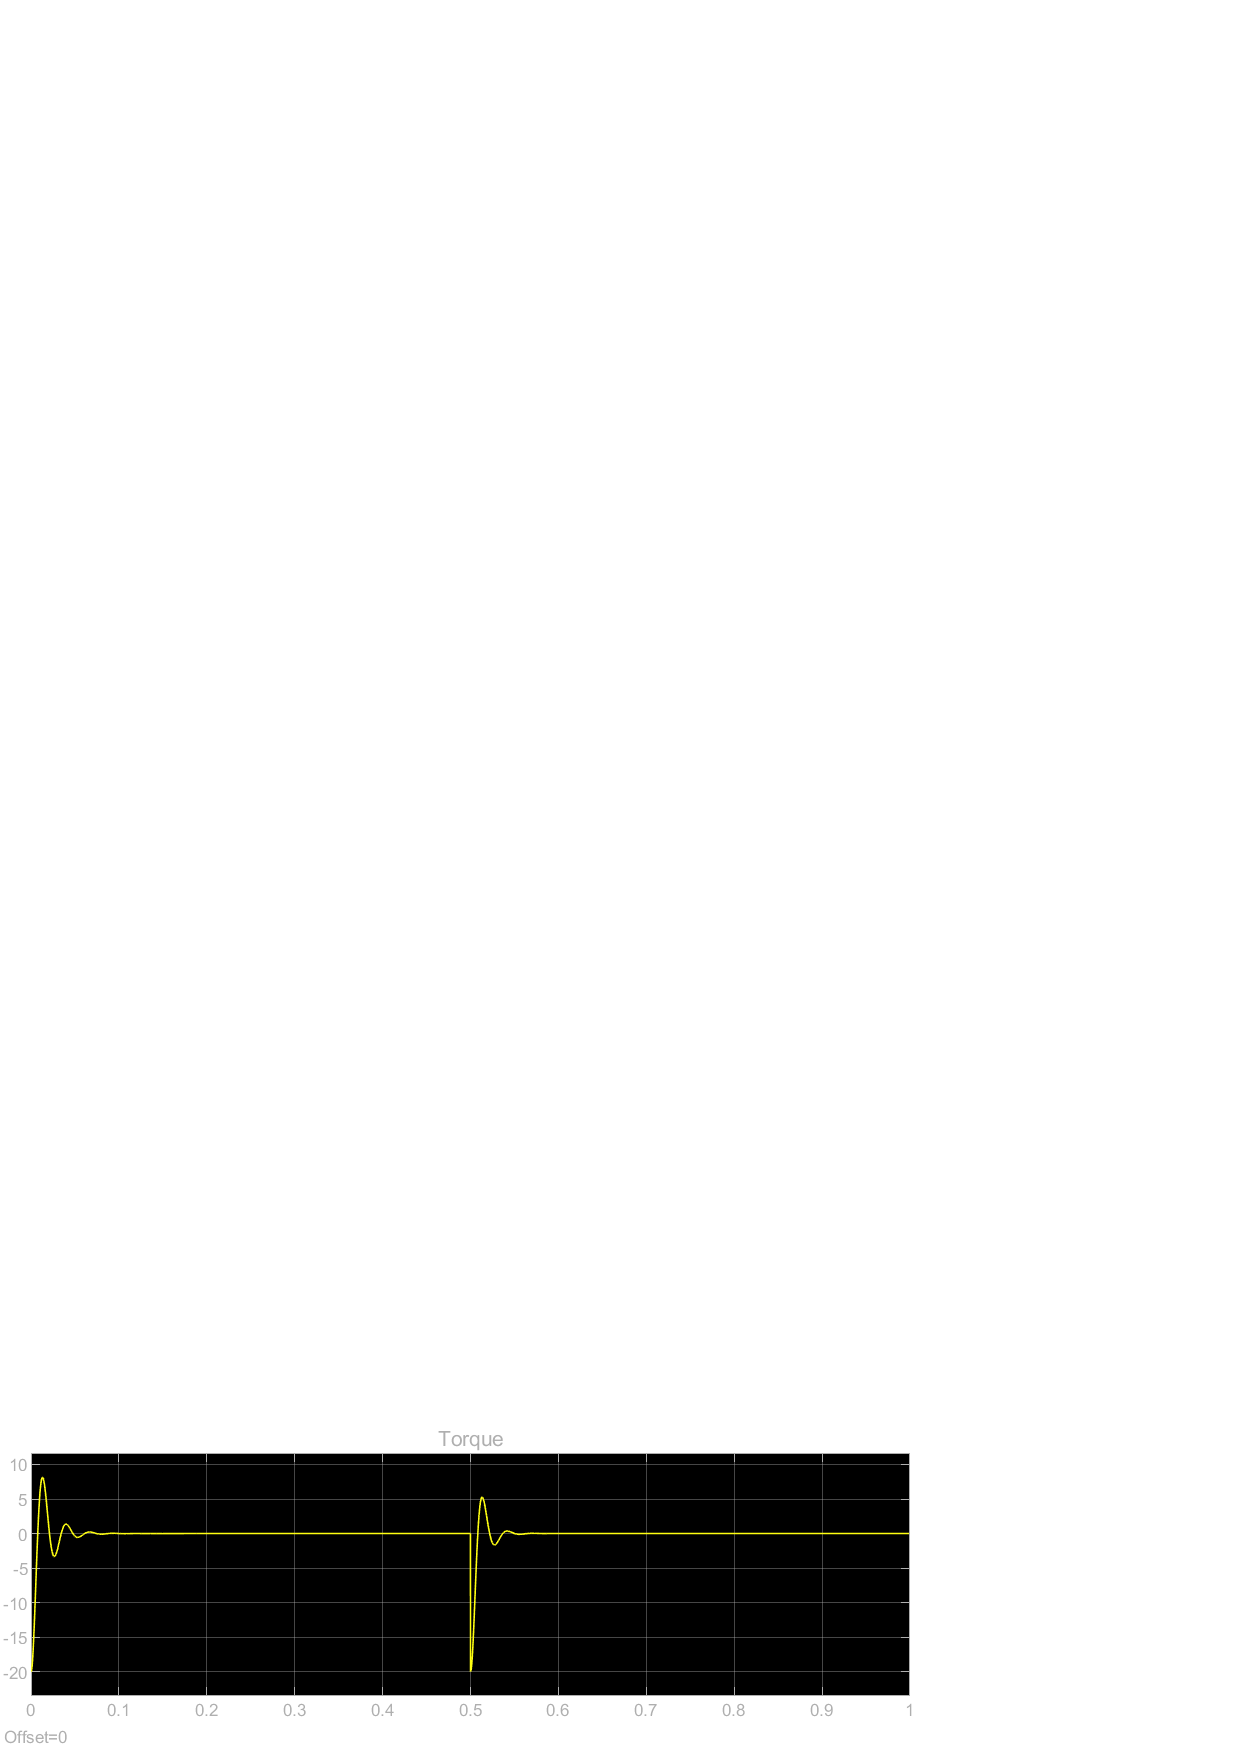
\includegraphics[width=1\linewidth]{pictures/control/torque.PNG}
	\caption{Simulink model of the motor with torque, rotational speed and the position of the rotor as output and the the d- and q-current as input.}
	\label{fig:torque_model}
\end{figure}

\subsubsection{Complete motor model}
The three models, for the d-direction, the q-direction and the mechanical part, are put into subsystems and connected as can be seen on figure \ref{fig:motor}.

\begin{figure}[H]
	\centering
	\includegraphics[width=1\linewidth]{pictures/control/motor_model.PNG}
	\caption{Simulink model of the full motor model.}
	\label{fig:motor}
\end{figure}

The motor model is in the dq-frame which means the three rotational phases voltages are converted to the dq-frame in the beginning of the model. The model outputs the d- and q-current, the torque, speed and angle of the motor. The rotational speed out of the motor model is the mechanical speed, and is therefore converted to the electrical speed before it is put into to the d- and q-models. 



\subsubsection{Control system}
\label{sec:control_system}

\begin{figure}[H]
	\centering
	\includegraphics[width=0.9\linewidth]{pictures/control/control_model.png}
	\caption{}
	\label{fig:control_system}
\end{figure}

\subsection{PI-controller}

To set the PI-controller the transfer functions for the d- and q-direction is determined, with the voltages as input and the current as output. This is done based on the equations for the voltages in the d- and q-direction, equation \ref{eq:d_direction} and \ref{eq:q_direction}.
Because a transfer function only can have one input and one output, the two equation, \ref{eq:d_direction} and \ref{eq:q_direction}, is shortened. The new equation can be seen in equation \ref{eq:d_direction3} and \ref{eq:q_direction3}.

\begin{equation}
    \label{eq:d_direction3}
    v_d = L_d \frac{d i_d}{dt} + R_s i_d
\end{equation}

\begin{equation}
    \label{eq:q_direction3}
    v_q = L_q \frac{d i_q}{dt} + R_s i_q
\end{equation}

As seen in the two equations, \ref{eq:d_direction3} and \ref{eq:q_direction3}, the parts in the equations depending on other variables than the current is neglected. 
This Laplace transformed and converted to the transfer functions for the two systems.

\begin{equation}
    \frac{I_d(s)}{V_d(s)} = \frac{ \frac{1}{ \frac{L_d}{R_s} } }{ \frac{R_s}{ \frac{L_d}{R_s} } + R_s s }
\end{equation}